\documentclass{beamer}

\usetheme{Madrid}

\usepackage{hyperref}
\usepackage{tikz}
\usetikzlibrary{arrows.meta}
\usetikzlibrary{positioning}
\usetikzlibrary{shapes, shapes.geometric}

\hypersetup{colorlinks=true, urlcolor=blue, linkcolor=white}
\urlstyle{same}
\definecolor{madridblue}{RGB}{0,114,198}
\newcommand{\colouredblock}[4]{%
  {\setbeamercolor{block title}{bg=#1!50, fg=#2}%
   \setbeamercolor{block body}{bg=#1!10, fg=#2}%
   \begin{block}{#3}%
   #4
   \end{block}%
  }%
}

\setbeamertemplate{itemize subitem}{\textbf{$\rightarrow$}}

\title[Doctor-patient matching \& scheduling]{Doctor-patient matching \& scheduling  \\optimisation problem}
\author[Peleg, Tyler \& Hamish]{Peleg Kark-Levin \and Tyler Pearn \and Hamish McKay}
\institute[UQ]{The University of Queensland}
\date{Semester 2, 2025}

\begin{document}
\begin{frame}
  \titlepage
  \vspace{-1em}
  \begin{figure}
      \centering
      \includegraphics[width=1\linewidth]{title_plot.png}
  \end{figure}
\end{frame}

\begin{frame}{Project overview}
\textbf{Goal:} Reproduce, improve, and extend the model presented \\ by Jiang et al. (2025)\footnote{\textbf{Reference:} Jiang et al. (2025). \textit{Logic-based Benders decomposition for doctor-patient matching and \\ scheduling considering chronic patients’ online consultation time preference}. Computers \& Operations Research 183: 107207. \url{https://doi.org/10.1016/j.cor.2025.107207}} on doctor-patient matching and scheduling for online consultations.

\vspace{1em}
\textbf{Problem summary:}  
\begin{itemize}
    \item Multi-objective optimisation: maximise patient satisfaction, doctor satisfaction, and number of appointments.
    \item Complex constraints: overlapping availability, consultation duration by disease/expertise, and individual preferences.
    \item High heterogeneity among patients and doctors → limited symmetry exploitation, tightly coupled problem.
\end{itemize}
\end{frame}

\begin{frame}{Modelling journey}
\begin{center}
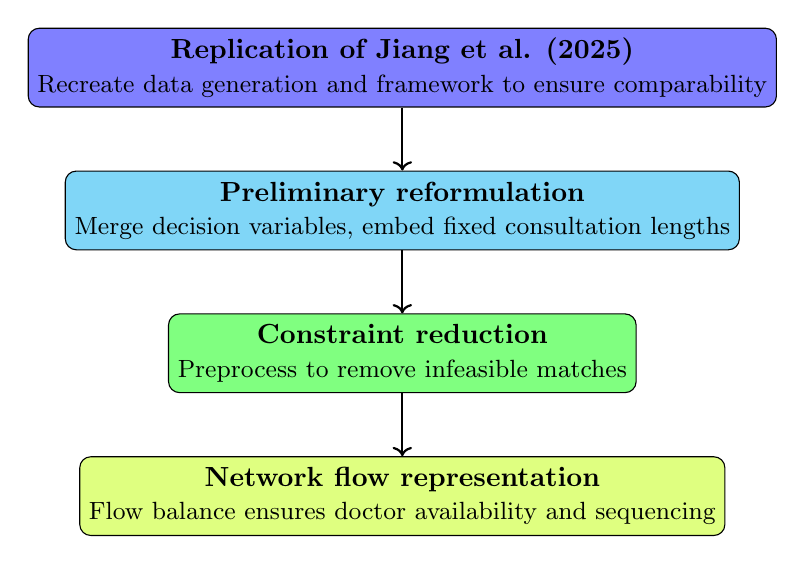
\begin{tikzpicture}[every node/.style={rectangle, draw, rounded corners, align=center, minimum width=4.5cm, minimum height=1cm}, node distance=0.8cm]

\node[fill=blue!50] (replication) {\textbf{Replication of Jiang et al. (2025)}\\\small Recreate data generation and framework to ensure comparability};
\node[fill=cyan!50, below=of replication] (reformulation) {\textbf{Preliminary reformulation}\\\small Merge decision variables, embed fixed consultation lengths};
\node[fill=green!50, below=of reformulation] (constraint) {\textbf{Constraint reduction}\\\small Preprocess to remove infeasible matches};
\node[fill=lime!50, below=of constraint] (network) {\textbf{Network flow representation}\\\small Flow balance ensures doctor availability and sequencing};

\draw[->, thick] (replication.south) -- (reformulation.north);
\draw[->, thick] (reformulation.south) -- (constraint.north);
\draw[->, thick] (constraint.south) -- (network.north);

\end{tikzpicture}
\end{center}
\end{frame}

\begin{frame}{Modelling journey (continued)}
\begin{center}
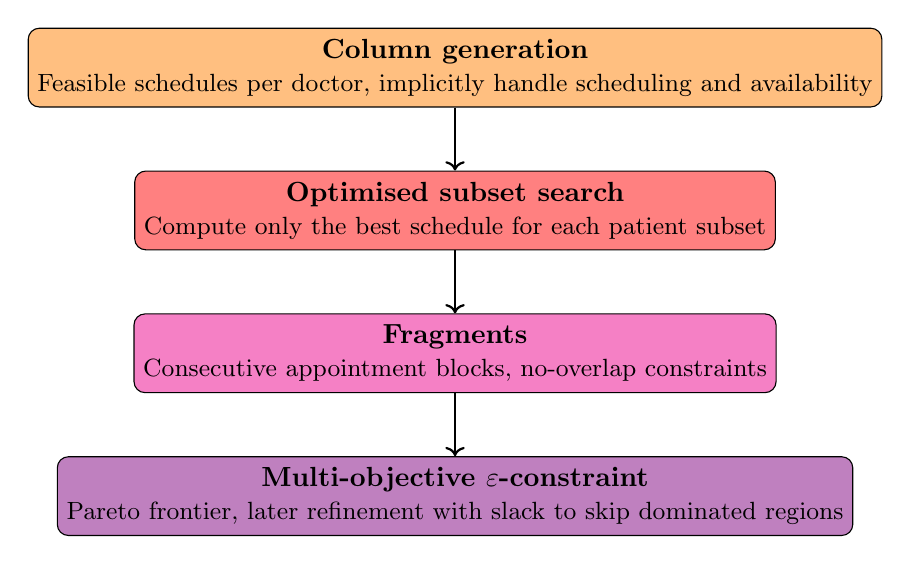
\begin{tikzpicture}[every node/.style={rectangle, draw, rounded corners, align=center, minimum width=4.5cm, minimum height=1cm}, node distance=0.8cm]

\node[fill=orange!50] (column) {\textbf{Column generation}\\\small Feasible schedules per doctor, implicitly handle scheduling and availability};
\node[fill=red!50, below=of column] (subset) {\textbf{Optimised subset search}\\\small Compute only the best schedule for each patient subset};
\node[fill=magenta!50, below=of subset] (fragments) {\textbf{Fragments}\\\small Consecutive appointment blocks, no-overlap constraints};
\node[fill=violet!50, below=of fragments] (epsilon) {\textbf{Multi-objective $\varepsilon$-constraint}\\\small Pareto frontier, later refinement with slack to skip dominated regions};

\draw[->, thick] (column.south) -- (subset.north);
\draw[->, thick] (subset.south) -- (fragments.north);
\draw[->, thick] (fragments.south) -- (epsilon.north);

\end{tikzpicture}
\end{center}
\end{frame}

\begin{frame}{Model outline}
    We model doctor-patient matching as a scheduling problem, \\balancing patient and doctor preferences across multiple \\time periods.

    \vspace{1em}
    \textbf{Sets:}    
    \begin{minipage}[t]{0.45\textwidth}
        \begin{itemize}
            \item[$I$] Patients
            \item[$J$] Doctors
            \item[$K$] Disease types
            \item[$T$] Time periods
            \item[$S$] Candidate schedules
        \end{itemize}
    \end{minipage}
    \begin{minipage}[t]{0.45\textwidth}
        \begin{itemize}
            \item[$I_k$] Patients with disease $k$
            \item[$J_k$] Doctors qualified for $k$
            \item[$\mathrm{treat}_{j,k}$] Treatment time for 
            doctor $j$ and disease $k$
            \item[$T^\mathrm{compatible}_{i,j}$] Feasible start times
            for patient $i$ and doctor $j$
        \end{itemize}
    \end{minipage}
    
    \vspace{1em}
    \textbf{Objectives:}
    \begin{itemize}
        \item Maximise patient satisfaction, number of appointments, and doctor satisfaction
    \end{itemize}
\end{frame}

\begin{frame}{Illustrative doctor–patient schedule}
    \textbf{Overview:}
    \begin{itemize}
        \item Each doctor is assigned a sequence of patients over time.
        \item Patient appointment times are shown in colour blocks.
    \end{itemize}    
    \begin{figure}
        \centering
        
\includegraphics[width=0.9\linewidth]{plot.png}
        \vspace{-1em}
        \caption{Example optimal schedule for 10 doctors and 100 patients}
        \label{fig:illustration}
    \end{figure}
\end{frame}

\begin{frame}{Baseline model}
    \begin{block}{Feasibility formulation}
        \textbf{Variables:}
        \begin{itemize}
            \item Appointment start times: 
            % $y_{i,j,t} \in \{0,1\}$: 1 if patient $i \in I$ is assigned to doctor $j \in J$ starting at time $t \in T$
            \[
            y_{i,j,t} \in \{0,1\} \qquad \forall i \in I, \;j \in J,\; t \in T
            \]
        \end{itemize}
        \textbf{Constraints:}
        \begin{itemize}
            \item Doctors not overbooked
            \item Patients assigned at most once
            \item Appointments in feasible time windows
            \item Only qualified doctor-disease assignments
        \end{itemize}
    \end{block}
\end{frame}

\begin{frame}{Preprocessed model}
    \begin{block}{Compatible times formulation}
        \textbf{Variables:}
        \begin{itemize}
            \item Appointment start times: 
            % $y_{i,j,t} \in \{0,1\}$: 1 if patient $i \in I_k$ with disease $k \in K$ is assigned to qualified doctor $j \in J_k$ starting at time $t \in T^\mathrm{compatible}_{i,j}$
            \[
            y_{i,j,t} \in \{0,1\} \qquad \forall k \in K, \;i \in I_k, \;j \in J_k, \;t \in T^\mathrm{compatible}_{i,j}
            \]
        \end{itemize}
        \textbf{Constraints:}
        \begin{itemize}
            \item Doctors not overbooked (sum over compatible times only)
            \item Patients assigned at most once (over compatible doctors and times)
        \end{itemize}
    \end{block}
\end{frame}

\begin{frame}{Network flow model}
    \begin{block}{Doctor available formulation}
        \textbf{Variables:}
        \begin{itemize}
            \item Appointment start times: 
            % $y_{i,j,t} \in \{0,1\}$: 1 if patient $i \in I_k$ with disease $k \in K$ is assigned to qualified doctor $j \in J_k$ starting at time $t \in T^\mathrm{compatible}_{i,j}$
            \[
            y_{i,j,t} \in \{0,1\} \qquad \forall k \in K, \;i \in I_k, \;j \in J_k, \;t \in T^\mathrm{compatible}_{i,j}
            \]
            % $z_{j,t} \in \{0,1\}$: 1 if doctor $j \in J$ is available to treat patients at time $t \in \mathrm{available}^\mathrm{doctor}_j$
            \item Doctor availability:
            \[
            z_{j,t} \in \{0,1\} \qquad \forall j \in J, \;t\in \mathrm{available}^\mathrm{doctor}_j
            \]
        \end{itemize}
        \textbf{Constraints:}
        \begin{itemize}
            \item Patients assigned at most once
            \item Doctor availability flows over time:
            \begin{itemize}
                \item $z_{j,t}$ updates based on previous availability and scheduled appointments
                \item Initial and final availability constraints ensure feasibility
            \end{itemize}
        \end{itemize}
    \end{block}
\end{frame}

\begin{frame}{Network flow model}
    \begin{block}{Doctor available formulation}
        Doctor availability flows over time:
        \begin{multline*}
            z_{j,t} = z_{j,t-1} 
            + \overbrace{\sum_{k \in D_j} \sum_{\substack{i \in I_k: \\ t^\mathrm{start}_{j,k} \in T^\mathrm{compatible}_{i,j}}} y_{i,j,t^\mathrm{start}_{j,k}}}^{\text{inflows}}
            - \overbrace{\sum_{k \in D_j} \sum_{\substack{i \in I_k: \\ t \in T^\mathrm{compatible}_{i,j}}} y_{i,j,t}}^{\text{outflows}} \\
            \qquad \forall j \in J,\; t \in \mathrm{available}^\mathrm{doctor}_j, t^\mathrm{start}_{j,k} = t - \mathrm{treat}_{j,k}
        \end{multline*}
    \end{block}
\end{frame}

\begin{frame}{Model building comparison}  
    \begin{figure}
        \centering
        
\includegraphics[width=1\linewidth]{before_presolve_summary.png}
        \caption{\centering Gurobi model building before presolve \\(averaged over 1000 iterations)}
        \label{fig:compact}
    \end{figure}
    \textbf{Key points:}
    \begin{itemize}
        \item The feasibility model has a longer set up time and is very sparse
        \item All three models give the exact same objective values
        \item Presolve removes the exact same number of rows and columns for each model
    \end{itemize}
\end{frame}

\begin{frame}{Performance profiles}
    \textbf{Overview:}
    \begin{itemize}
        \item The feasibility model has the steepest slope, with the \\least variability in solving times across different seeds
        \item The doctor available model performs best overall, with most instances solved to optimality in the shortest amount of time
    \end{itemize}    
    \begin{figure}
        \centering
        
\includegraphics[width=1\linewidth]{graph_1000_seed_model_results.png}
        \vspace{-1em}
        \caption{\centering Performance profiles for compact IP models \\(1000 instances with 100 patients, 10 doctors, 4 diseases, and 20 time periods)}
        \label{fig:profiles}
    \end{figure}
\end{frame}

\begin{frame}{Huge model}
    We developed a huge integer program that selects one \\feasible schedule per doctor, each representing a full \\sequence of patient appointments
    \begin{figure}
        \centering
        
\includegraphics[width=0.9\linewidth]{plot_schedule.png}
        \vspace{-1em}
        \caption{Example schedule for a doctor}
        \label{fig:schedule}
    \end{figure}
\end{frame}

\begin{frame}{Huge model}
    \begin{block}{Doctor schedule formulation}
        \textbf{Variables:}
        \begin{itemize}
            \item Doctor schedules: 
            \[
            z_{j,s} \in \{0,1\} \qquad \forall j \in J, \; s \in S_j
            \]
            where $S_j$ is the subset of feasible schedules for doctor $j$
            % 1 if doctor $j$ is assigned schedule $s$ (sequence of patients + appointment times)
        \end{itemize}
        \textbf{Constraints:}
        \begin{itemize}
            \item Doctors assigned at most one schedule
            \item Patients assigned at most once
        \end{itemize}
    \end{block}
\end{frame}

\begin{frame}{Huge model}
    \begin{block}{Doctor schedule formulation}
        \textbf{Constraints:}
        \begin{itemize}
            \item Doctors assigned at most one schedule
            \begin{equation*}
                \sum_{s\in S_j } z_{j,s} = 1 \qquad \forall j \in J
            \end{equation*}
            \item Patients assigned at most once
            \begin{equation*}
                \sum_{j \in J} \sum_{s\in S_j\;|\; i\in S_j} z_{j,s} \le 1 \qquad \forall i \in I
            \end{equation*}
        \end{itemize}
    \end{block}
\end{frame}

\begin{frame}{Generating candidate schedules}
    \begin{block}{Naive exhaustive search}
    Enumerate all feasible sequences of patients and start times \\for each doctor \textit{a priori}, and compute objective contributions for each schedule   
    \begin{itemize}
        \item Problem: combinatorial explosion even for small instances
    \end{itemize}
    \end{block}
    \vspace{1em}
    \textbf{Observation:} many schedules are dominated by others
    \begin{itemize}
        \item For schedules for a doctor that include the same patients:
        \begin{itemize}
            \item The number of appointments and doctor satisfaction are identical
            \item Only patient satisfaction may differ
        \end{itemize}
        \item Schedules with strictly lower patient satisfaction can be discarded
    \end{itemize}
\begin{figure}
    \centering
    \includegraphics[width=0.75\linewidth]{schedule_for_cg.png}
    \caption{Every valid permutation of these appointments are generated, where one has the highest patient satisfaction}
    \label{fig:schedule_for_cg}
\end{figure}
\end{frame}

\begin{frame}{Optimised subset search}
    \textbf{Key idea:}
    \begin{itemize}
        \item Enumerate all feasible \textbf{subsets of patients} for each doctor
        \item For each subset, find the schedule that maximises patient satisfaction
        \item Only keep \textbf{non-dominated schedules}
    \end{itemize}
    \begin{block}{Column generation algorithm}
    \begin{itemize}
        \item Start with single-patient schedules
        \item Iteratively build larger sets by adding patients
        \item Solve small IP (using one of the compact formulations) for each subset to find best schedule
        \item Stop when no new feasible schedules can be generated
    \end{itemize}
    \end{block}
\end{frame}

\begin{frame}{Column generation time}
    \begin{figure}[h]
        \centering
        
\includegraphics[width=0.6\linewidth]{smart_cg_times.png}
        \vspace{-1em}
        \caption{\centering Average generation time vs number of patients \\ (5 doctors, 2 diseases, 20 time periods)}
        \label{fig:smart_cg_times}
    \end{figure}
    Naive ran for 5 patients and generates 122176 schedules. The subset method generates for 25 patients, 145553 schedules.
\end{frame}

\begin{frame}{Multi-processing}
    \begin{figure}[h]
        \centering
        \includegraphics[width=0.7\linewidth]{multi-processing.png}
        \vspace{-1em}
        \caption{\centering Performance profiles for column generation procedures \\(100 instances with 20 patients, 5 doctors, 4 diseases and 10 time periods)}
        \label{fig:multiprocessing}
    \end{figure}
\end{frame}

\begin{frame}{Generating schedule fragments}
    We explored the idea of generating \textbf{schedule fragments} as consecutive appointment blocks, to reduce the size of the columns generated

    \vspace{1em}
    \textbf{Key features:}
    \begin{itemize}
        \item Each fragment represents a feasible mini-schedule of \\consecutive appointments for a single doctor
        \item Start times are explicitly specified to ensure appointments align without gaps or overlaps
        \item Fragments can later be linked to form full schedules that respect availability and treatment lengths
        \item Must generate fragments for each doctor separately because doctors take different amounts of time to treat diseases
    \end{itemize}
\end{frame}

\begin{frame}{Fragments model}
    \begin{figure}
        \centering
        
\includegraphics[width=0.9\linewidth]{plot_fragment.png}
        \vspace{-1em}
        \caption{Example fragments of a doctor's schedule}
        \label{fig:fragments}
    \end{figure}
\end{frame}

\begin{frame}{Fragments model}
    \begin{block}{Doctor schedule fragments formulation}
        \textbf{Variables:}
        \begin{itemize}
            \item Doctor schedules: 
            \[
            w_{j,f} \in \{0,1\} \qquad \forall j \in J, \; f \in F_j
            \]
            where $F_j$ is the subset of feasible fragments for doctor $j$
            % 1 if doctor $j$ is assigned fragment $f$ (sequence of patients + appointment times)
        \end{itemize}
        \textbf{Constraints:}
        \begin{itemize}
            \item Patients assigned at most once
            \item No overlap (over fragments)
        \end{itemize}
    \end{block}
\end{frame}

\begin{frame}{Multi-objective optimisation}
    We aim to maximise three objectives simultaneously:
    \begin{align*}
        \max \quad & f_0(x) && \text{(Patient satisfaction)} \\
        \max \quad & f_1(x) && \text{(Total appointments)} \\
        \max \quad & f_2(x) && \text{(Doctor satisfaction)}
    \end{align*}
    subject to feasibility constraints $x \in \mathcal{X}$.

    \begin{block}{Epsilon-constraint method}
        \begin{itemize}
            \item Choose one objective ($f_0$) as primary
            \item Convert the others into constraints:
            \[
            f_1(x) \geq \varepsilon_1, \quad f_2(x) \geq \varepsilon_2
            \]
            \item Vary $(\varepsilon_1,\varepsilon_2)$ over feasible ranges to trace the trade-offs
            \item Pareto filtering then identifies non-dominated (efficient) solutions
        \end{itemize}
    \end{block}
\end{frame}


\begin{frame}{Pareto frontier}
    \begin{block}{Dense grid search}
        \begin{itemize}
            \item Iterates through all $(\varepsilon_1,\varepsilon_2)$ pairs, guarantees full Pareto coverage
            \item[$\star$] Many redundant solves in dominated regions
        \end{itemize}
    \end{block}

    \begin{columns}[T]
    \column{0.5\textwidth}

    \begin{block}{Slack-based search}
        \begin{itemize}
            \item Uses \textbf{slack values} $s_i = f_i(x^*) - \varepsilon_i$ to skip ahead by $\lfloor s_i / \Delta_i \rfloor$ steps
            \item Reduces computational effort by avoiding already-covered areas
            \item Idea: reuse ``information" from prior solves to accelerate the search
        \end{itemize}
    \end{block}

    \column{0.45\textwidth}
    \vspace{1em}
    \centering
    % \caption{Epsilon-constraint methods}
    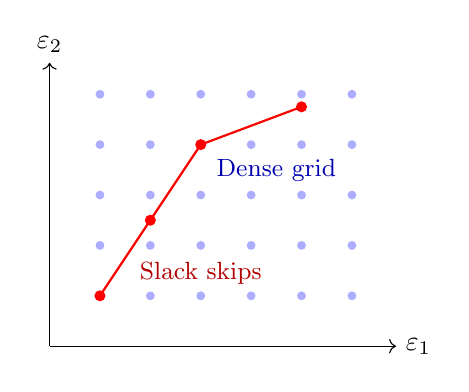
\begin{tikzpicture}[scale=0.8]
        \draw[->] (0,0) -- (5.5,0) node[right] {$\varepsilon_1$};
        \draw[->] (0,0) -- (0,4.5) node[above] {$\varepsilon_2$};

        % Dense grid
        \foreach \x in {1,2,3,4,5,6}
            \foreach \y in {1,2,3,4,5}
                \fill[blue!40, opacity=0.8] (\x*0.8,\y*0.8) circle (2pt);

        % Slack path
        \draw[-, thick, red] (0.8,0.8) -- (1.6,2) -- (2.4,3.2) -- (4,3.8);
        \foreach \p in {(0.8,0.8),(1.6,2),(2.4,3.2),(4,3.8)}
            \fill[red] \p circle (2.5pt);

        \node[blue!70!black] at (3.6,2.8) {\small Dense grid};
        \node[red!70!black] at (2.4,1.15) {\small Slack skips};
    \end{tikzpicture}
    \end{columns}
\end{frame}

\begin{frame}{Sketching the Pareto frontiers}
    \textbf{Overview:}
    \begin{itemize}
        \item Each point represents a feasible solution obtained from \\the multi-objective model 
        \item The frontier traces the trade-offs between objectives, showing where improving one comes at the cost of another
        % \item Dominated solutions (grey) are filtered out, leaving only the efficient frontier (coloured)
    \end{itemize}    
    \begin{figure}
        \centering
        
\includegraphics[width=\linewidth]{pareto_slack_2d_with_dominated.png}
        \vspace{-2em}
        \caption{Example Pareto frontier diagrams for objective pairs}
        \label{fig:2d}
    \end{figure}
\end{frame}

\begin{frame}{Implementation notes}
    \textbf{Results and challenges}
    \begin{itemize}
        \item The dense grid method works reliably and generates a complete Pareto frontier
        \item The slack-based approach has been implemented but currently shows inconsistent skipping behaviour
    \end{itemize}
    \begin{block}{Next steps}
        \begin{itemize}
            \item Debug slack update rules to ensure consistent skipping, by checking whether a potential $(\varepsilon_1,\varepsilon_2)$ pair is \textit{un-dominated} before optimising
            \item Validate correctness by comparing recovered frontier with dense search results
        \end{itemize}
    \end{block}
\end{frame}

\begin{frame}{Ideas}
    \begin{itemize}
        \item \textbf{Partial column generation:} apply different solution \\methods for different doctor types within the one IP
        \begin{itemize}
            \item For lowly available and slow doctors, use the huge formulation (since the schedules can be generated very fast)
            \item For highly available and fast doctors, use a compact IP formulation or fragments to solve directly
        \end{itemize}
    \end{itemize}
    \begin{figure}
        \centering
        
\includegraphics[width=1\linewidth]{bad_doctor_good_doctor.png}
        \vspace{-2em}
        \caption{Lowly available vs. highly available doctors}
        \label{fig:bad_good}
    \end{figure}
\end{frame}

\begin{frame}{Ideas}
    \begin{itemize}
        \item \textbf{Benders' decomposition:} master problem matches \\patients to doctors, sub-problem schedules those \\ patients who have been matched (similar to paper but simplified)
        \begin{itemize}
            \item Master problem ensures doctors are qualified and time windows are compatible
            \item Feasibility cuts ensure that subsets of patients can indeed be served a doctor (i.e. patients can be arranged within the doctor's availability)
            \item Optimality cuts ensure additional patients in a given subset increase the objective value for patient satisfaction; the other objective values are taken care of by the epsilon-constraint method
        \end{itemize}
    \end{itemize}
    \vspace{-2em}
    \centering
    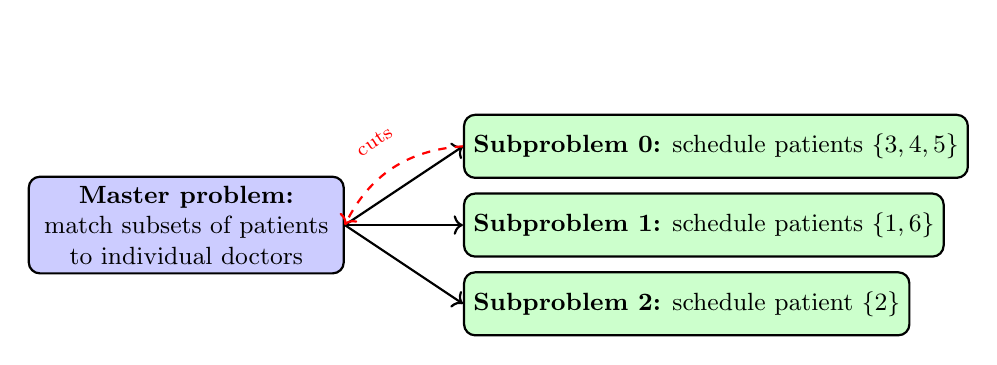
\begin{tikzpicture}[
        node distance=1.5cm,
        every node/.style={rectangle, draw, rounded corners, align=center, minimum width=4cm, minimum height=0.8cm, font=\small, thick},
        arrow/.style={->, thick}
    ]
    
    % Master problem
    \node[fill=blue!20] (mp) {\textbf{Master problem:}\\match subsets of patients\\to individual doctors};
    
    % Subproblems
    \node[fill=green!20, right=of mp, yshift=1cm] (sp1) {\textbf{Subproblem 0:} schedule patients $\{3, 4, 5\}$};
    \node[fill=green!20, right=of mp] (sp2) {\textbf{Subproblem 1:} schedule patients $\{1, 6\}$};
    \node[fill=green!20, right=of mp, yshift=-1cm] (sp3) {\textbf{Subproblem 2:} schedule patient $\{2\}$};
    
    % Arrows
    \draw[arrow] (mp.east) -- (sp1.west);
    \draw[arrow] (mp.east) -- (sp2.west);
    \draw[arrow] (mp.east) -- (sp3.west);
    
    % Feedback arrows (optional, for cuts)
    \draw[arrow, dashed, color=red] (sp1.west) to[bend right=30] node[draw=none, fill=none, above, sloped, color=red, font=\scriptsize]{cuts} (mp.east);
    % \draw[arrow, dashed] (sp2.west) to[bend right=5] (mp.east);
    % \draw[arrow, dashed] (sp3.west) to[bend left=10] (mp.east);
    
    \end{tikzpicture}
\end{frame}

\begin{frame}{Thank you}
  \textbf{Reference:} Jiang et al. (2025). \textit{Logic-based Benders decomposition for doctor-patient matching and scheduling considering chronic patients’ online consultation time preference}. Computers \& Operations Research 183: 107207. 
  \url{https://doi.org/10.1016/j.cor.2025.107207}
\end{frame}

\end{document}
